%!TEX root = ../report.tex

% 
% Related work
% 

\section{Related Work}


The following section starts to present the use of refactoring tools and an overview of static refactoring tools.
After that it presents the refactoring tools for the dynamic languages such as, Scheme, JavaScript, Smalltalk, Python and Racket.
Then it presents multi-language refactorings.
Finally it has a conclusion about the related work.

%How we Refactor, and how we know it.
\subsection{Use of static refactoring tools}

Understanding how users refactor and use refactoring tools is an important step to better improve the refactoring tools.
The information necessary to reason about how the users refactor was gathered by collecting some data sets \cite{murphy2012we}.


%Murphy et al \cite{murphy2012we} collected some data sets in order to understand how the users refactor.
The User data set was collected \cite{murphy2006java} in 2005, it has records of 41 volunteer programmers using eclipse which 95\% of them programmed in Java. %Whit this we implied that Refactoring tools are underused [10]

The Everyone data set was collected from the Eclipse Usage Collector, the data used aggregates activity from over 13000 Java developers between 04/08 to 01/09 and it also includes non-Java developers.

The Toolsmiths data set that consists in information about 4 developers who primarily maintain eclipse's refactoring tools from 12/05 to 08/07. 
However, it is not publicly available and is not described in other papers.
There is only a similar study \cite{robbes2007mining} that uses data from the author and another developer. 


%Many other authors have mined software repositories automatically for refactorings (WeiBgerber and Diehl [18]) they did not know of other research that compares refactoring tool logs with code histories.
Using all the data sets it is possible to see which are the most common refactoring operations used by the users and they are: rename, extract local variable, inline, extract method and move. The sum of the use percentages of this refactoring operations is between 86.4\% and 92\% of the data sets. % 86.4 90.8 92.0 

However the refactoring behavior differs among users. The most used refactoring operations is the rename for all the sets, but the used percentage drastically differs between Toolsmiths and the other sets. Toolsmiths usage of the rename refactoring is 29\% while the User set and Everyone set is 62\% and 75\% respectively.

Using the data sets of Users and Toolsmiths it was possible to confirm that refactoring operations are frequent. 
In the Users data set, 41\% of programming sessions contained refactoring activities and the sessions that did not have refactoring activities were the sessions where less edits where made.
In the toolsmith data set only 2 weeks of the year 2006 did not had any refactoring operation and, in average, it had 30 refactoring operations per week. 
In 2007 every week had refactoring activities and the average was 47 refactoring operations a week.

Besides refactoring operations being frequent, the refactoring tools are underused. 
%In order to decide whether the refactoring operation was manual or tool assisted they tried to correlate refactoring activities with tool support. 
%If the refactoring activities is correlated with tool support it is classified as being a tool assisted refactoring.
After evaluating the refactoring activities in the data set they were unable to link 73\% of the refactoring operations to a tool supported refactoring. 
All this numbers are computed from the Toolsmiths data set which is in theory the group who knows and better uses the refactoring tools.


\subsection{Overview of static Refactoring tools}
%\textbackslash
\begin{table}
\caption{Refactoring operations available by default}
\label{tab-Comparing-Static}
\begin{tabular}{|l|c|c|c|c|c|c|}
\hline\noalign{\smallskip}
Refactoring \textbackslash IDE           & Visual Studio & Eclipse & CDT & IntelliJ & NetBeans & Jbuilder \\
\noalign{\smallskip}
\hline
\noalign{\smallskip}
Rename                    & x             & x       & x   & x        & x        & x        \\ \hline
Move                      &               & x       & x   & x        & x        & x        \\ \hline
Change method signature   &               & x       &     & x        &          &          \\ \hline
Extract method            & x             & x       & x   & x        &          & x        \\ \hline
Extract local variable    &               & x       &     & x        &          & x        \\ \hline
Extract constant          &               & x       & x   & x        &          &          \\ \hline
Inline                    &               & x       &     & x        & x        &          \\ \hline
To nested 			      &               & x       &     & x        &          &          \\ \hline
Move type to new file     &               & x       &     & x        &          &          \\ \hline
Variable to field         &               & x       &     & x        &          &          \\ \hline
Extract superclass        &               & x       & x   & x        & x        &          \\ \hline
Extract interface         & x             & x       &     & x        & x        &          \\ \hline
Change to supertype 	  &               & x       &     &          & x        &          \\ \hline
Push down                 &               & x       &     & x        & x        &          \\ \hline
Pull up                   &               & x       &     & x        & x        &          \\ \hline
Extract class             &               & x       &     & x        &          &          \\ \hline
Introduce parameter       &               & x       &     & x        & x        &          \\ \hline
Introduce indirection     &               & x       &     &          &          &          \\ \hline
Introduce factory         &               & x       &     & x        & x        &          \\ \hline
Encapsulate field         & x             & x       &     & x        &          &          \\ \hline
Generalize declared type  &               & x       &     &          &          &          \\ \hline
Type Migration            &               &         &     & x        &          &          \\ \hline
Remove Middleman          &               &         &     & x        &          &          \\ \hline
Wrap Return Value         &               &         &     & x        &          &          \\ \hline
Safe Delete               &               &         &     & x        & x        &          \\ \hline
Replace Method duplicates &               &         &     & x        &          &          \\ \hline
Static to instance method &               &         &     & x        &          &          \\ \hline
Make Method Static        &               &         &     & x        &          &          \\ \hline
Change to interface 	  &               &         &     & x        &          &          \\ \hline
Inheritance to delegation &               &         &     & x        &          &          \\ \hline
\end{tabular}
\end{table}
 
\begin{table}[htbp]
\caption{Refactoring operations definitions:}
\label{tab-Refactoring-Definitions}
\begin{tabular}{ p{2.95cm}| p{9.15cm}}
\hline\noalign{\smallskip}
Refactoring name 		  & Definition \\
\noalign{\smallskip}
\hline
\noalign{\smallskip}
Rename                    & Renames the selected element and corrects all references.                                                                                                                 \\ \hline
Move                      & Moves the selected elements and corrects all references.                                                                                                                  \\ \hline
Change signature          & Change parameter names, types and updates all references.                                                                                                                 \\ \hline
Extract method            & Creates a new method with the statements or expression selected and replaces with a reference to the new method.                                                          \\ \hline
Extract local variable    & Creates a new variable assigned to the expression selected and replaces with a reference to the new variable.                                                             \\ \hline
Extract constant          & Creates a static final field from the selected expression.                                                                                                                \\ \hline
Inline                    & Inline local variables, methods or constants.                                                                                                                             \\ \hline
To nested                 & Converts an anonymous inner class to a member class.                                                                                                                      \\ \hline
Move type to new file     & Creates a new compilation unit and updates all references.                                                                                                                \\ \hline
Variable to field         & Turn a local variable into a field.                                                                                                                                       \\ \hline
Extract superclass        & Creates a new abstract class, changes the current class to extend the new class and moves the selected methods and fields to the new class.                               \\ \hline
Extract interface         & Creates a new interface and makes the class implement it.                                                                                                                 \\ \hline
Change to Supertype       & Replaces, where it is possible, all occurrences of a type with one of its supertypes.                                                                                     \\ \hline
Push down                 & Moves a set of methods and fields from a class to its subclasses.                                                                                                         \\ \hline
Pull up                   & Moves a field or method to a superclass, if it is a method, declares the method as abstract in the superclass.                                                            \\ \hline
Extract class             & Replaces a set of fields with new container object.                                                                                                                       \\ \hline
Introduce parameter       & Replaces an expression with a reference to a new method parameter and updates all callers of the method.                                                                  \\ \hline
Introduce indirection     & Creates an indirection method delegating to the selected method.                                                                                                          \\ \hline
Introduce factory         & Creates a new factory method, which calls a selected constructor and returns the created object.                                                                          \\ \hline
Encapsulate field         & Replaces all references to a field with getter and setter methods.                                                                                                        \\ \hline
Generalize type           & Allows the user to choose a supertype of the selected reference.                                                                                                          \\ \hline
Type Migration            & Change a member type and data flow dependent type entries.                                                                                                                \\ \hline
Remove Middleman          & Replaces all calls to delegating methods with the equivalent calls.                                                                                                       \\ \hline
Wrap Return Value         & Creates a wrapper class that includes the current return value.                                                                                                           \\ \hline
Safe Delete               & Finds all the usages or, simply delete if no usages found.                                                                                                                \\ \hline
Replace duplicates        & Finds all the places in the current file where the selected method code is fully repeated and change to corresponding method calls.                                      \\ \hline
Static to instance        & Converts a static method into an instance method with an initial method call argument being a prototype of newly created instance method call qualifier.                  \\ \hline
Make Method Static        & Converts a non-static method into a static one.                                                                                                                           \\ \hline
Change to Interface       & Used after using Extract an Interface it search for all places where the interface can be used instead of the original class.                                             \\ \hline
Inheritance to delegation & Delegate the execution of specified methods derived from the base class/interface to an instance of the ancestor class or an inner class implementing the same interface. \\ \hline
\end{tabular}
\end{table}
%Por C++ e comparar ve o que o eclipse tem.
The {\bf table.~\ref{tab-Comparing-Static}} compares this refactoring tools with each other and the Refactoring definitions, that were taken from Eclipse\footnote{help.eclipse.org/luna/topic/org.eclipse.jdt.doc.user/reference/ref-menu-refactor.htm} and IntelliJ\footnote{https://www.jetbrains.com/idea/features/refactoring.html} can be found on the {\bf table.~\ref{tab-Refactoring-Definitions}}.

The {\bf table.~\ref{tab-Comparing-Static}} compares the Visual Studio refactoring operations for C\# with Refactoring tools that have refactoring operations for Java because the languages are similar. It also compares with the Eclipse CDT  refactoring operations for C++ because in some aspects the languages are similar and the refactoring operations compared are similar to the refactoring operations for Java or C\#. 
The table only lists the refactoring operations that each IDE has by default in order to have a fairer way to compare them with each other.
It is easy to see that IntelliJ has almost all the refactoring operations in this table, followed by Eclipse and NetBeans.
However, even having significantly less refactoring operations available by default than the other tools, JBuilder has the most used ones as shown above.
Only Visual Studio has 2 out of 5 most used refactoring operations available by default, but there are easily installed plug-ins that cover the more important refactoring operations. 

%It is easy to see all the effort to provide to the programmers refactoring operations to help them refactoring their projects. 


\subsection{Haskell}

The HaRe system is a refactoring tool for Haskell that integrates with Emacs and Vim.
This tool was made for the working programmers instead of being a prof of concept prototype and it is implemented in Haskell.

The HaRe system also allows the users to design their own refactorings using the HaRe API.

\subsubsection{Representation}
\hfill \break

The HaRe \cite{thompson2005refactoring} system uses an AST of the program to be refactored in order to reason about the transformations to do.
The system also have a token stream in order to preserve the comments and the program layout by keep information about the source code location and the comments of all tokens.

\subsubsection{Stages of Refactoring}
\hfill \break

{\bf Information gathering and condition checking:} The Refactoring will only be performed if it preserves the semantics of the program.
It is needed some information, such as a set of identifiers of the scope, that information is gathered trough transversing the AST.

{\bf Transformation:} After the conditions are verified, it is possible to apply the refactoring operation, which is a transformation of the AST.

{\bf Program rendering:} After the refactoring operation the source code of the new program needs to be generated, keeping the original program layout as much as possible.

%insert pic?
\begin{figure}[h!]
  \centering
  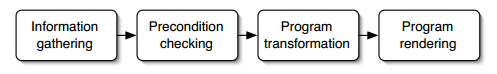
\includegraphics[width=0.75\textwidth]{img/HaReStagesOfRefactoring.png}
  \caption{Stages of Refactoring}
  \label{fig:HaReStages}
\end{figure}
%add structural refactorings, module-aware? 

\subsubsection{Refactorings Available} %review and change title
\hfill \break

Initially the HaRe system only had structural refactorings. 
Structural refactorings care about the objects defined in the program, the name and the scope of those objects. Examples of this are: Delete, Duplicate, Rename, Promote, Demote, etc \ldots
Then it was added module awareness to those refactorings. 
Module awareness is important because in Haskell it is possible to import definitions from other modules.
With module awareness it was possible to add new refactorings to the module like Clean the imported list, move a definition to another module or add and remove items of the export list.


\subsection{Scheme}
%Griswold
%Characteristics Dynamic language, Simple refactoring operations, Only One language, AST?, PDG?, Easy to create new operations?

Griswold \cite{griswold1991program} proved that meaning-preserving restructuring can substantively reduce the maintenance cost of a system.
A prototype was created to prove the concept, by creating restructuring operations for the Scheme programming language implemented in Common Lisp.
The prototype was developed for Scheme because of it's imperative features, simple syntax and it was available a (program dependence graph) PDG for Scheme implemented in Common Lisp
The prototype had simple restructuring operations to prove the concept, such as: moving an expression, renaming a variable, abstracting an expression, extracting a function, scope-wide function replacement, adding a reference indirection and adding looping to list references.

\subsubsection{Tool aided vs Manual Restructuring}
Griswold starts comparing automated restructuring with manual restructuring. 
To do that Griswold creates an experience.
It was given an initial program and a description of four transformations goals to six subjects.%An initial program and a description of the four goals of the transformations to be made was presented to 6 subjects. 

Although it was a experience with a small number of subjects, Griswold took several conclusions on how people manually restructure programs.
People use the copy/paste and the cut/paste paradigm to do the transformations. 
This means that they copy or cut the code and then paste it in the desired location.
Although the Cut/Paste paradigm is more dangerous because it is a destructive operation. 
This means if the user makes any error it is more difficult to correct it because it is a destructive operation.

Griswold also conclude that people make mistakes even with small and simple programs. 
And the cost of correcting mistakes is higher than the time to do the restructuring itself. 
And it also conclude that manual restructuring is haphazard. 
Meaning that the transformations were done in almost a random way when compared to the computer-assisted process.


\subsubsection{Architecture}

In order to be able to correctly implement these operations it was used contours and a PDG (program dependence graph).

The main program representation is the contours. 
Contours are an abstraction of the essential semantic properties that the AST (abstract syntax tree) represents in an efficient and complete form.

Whereas the PDG explicitly represents the key relationship of dependence between the operations in the program. 
The PDG is used because simple graph algorithms can extract this information and it has been a popular program representation for aiding program parallelization, optimization and version merging.
This features combined with the right semantic support make the PDGs a good foundation for preserving meaning during restructuring.
With these structures it is possible to combine them and have a single formalism to reason effectively about flow dependencies and scope structure.

%It is possible to have this representation because it have access to everything like a compiler does, and it tries to used work done, such as using a library for the PDG. Using DrRacket the semantic part is covered by the arrows created which helps having the semantic logic between things.






\subsection{Smalltalk}%add more?

The Refactoring Browser \cite{roberts1997refactoring} is a refactoring tool for smalltalk programs which goal was to make refactoring known and used by everyone.
to quote them  \textit{"The goal of our research is to move refactoring into the mainstream of program development. The only way this can occur is to present refactorings to developers in such a way that they cannot help but use them".} 

To do that they implemented the refactoring browser with the concern that the refactoring operations did by the programmer using the refactoring browser needed to be faster then by hand.

It was considered that the user of this tool is intelligent therefor automated refactorings would not suit them. 
Automated refactorings do not suit the user because they could generate code that does not make sense in the domain.
For example, the tool would generate new classes in order to eliminate duplicated code, by creating an abstract class, which might not make sense in the domain. Instead of doing that, the tool points out possible refactoring operations and let the user decide whether or not to do those operations.

In order to ensure behavior preservation the tool checks the preconditions of each refactoring before execution. 
However, there are some conditions that are more difficult to determine statically, such as dynamic typing and cardinality relationships between objects. 
Instead of checking the precondition statically the refactoring browser checks the preconditions dynamically. 

The preconditions checks are done using method wrappers to collect runtime information. 
The Refactoring Browser starts by doing the refactoring operation and then it adds a wrapper method to the original method. 
While the program is running, the wrapper detects the source code that called the original method and change it for the new method.
For example, in the rename refactoring, after applying the rename and while the program is running, whenever the old method is called, the browser suspends the execution and changes the code that called the old method by the new method. 

The problem of this approach is that the dynamically analysis is only as good as the test suit used by the programmer.


%%!TEX root = ../../report.tex

\subsection{Safe Refactoring}

Usually each refactoring contains a number of preconditions in order to preserve the behavior of the program, however most refactoring tools do not implement all preconditions because formally establishing all of them is not simple and refactoring tools allow wrong transformations with no warnings to the user.

One way to guarantee the preservation of the program behavior is using tests, but often tests suits do not catch the behavior changes and they might also be refactored by the tools since they use the program structure that is being transformed.

So Soares, Gustavo, et al. \cite{soares2010making} created a tool for eclipse that receives the source code that a refactroring is applied to, generates unit tests to the code being refactored and in the end it reports if the refactoring is safe to apply or not.

It uses a static analysis that identifies methods in common, a method to be considered that needs to have exactly the same modifier, return type, qualified name, parameters types and exceptions thrown in source and target programmers.
After identifying those methods it uses Randoop \cite{pacheco2007feedback},  %ADD CITATION
 a tool that generates unit tests for classes within a time limit.

Some dynamic refactoring tools such as Smalltalk refactoring browser and similar ones would improve and remove the test suit limitation by being paired with a tool like this one. However that level of static analysis is not that trivial to achieve and that is a big problem. %throwback 
However there is already a tool \cite{soares2010making} for Eclipse that receives the source code that a refactoring is applied to, generates unit tests to the code being refactored and at the end it reports if the refactoring is safe to apply or not.

The tool uses a static analysis that identifies methods that have exactly the same modifier, return type, qualified name, parameters types and exceptions thrown in source and target programmers.
After identifying those methods it uses Randoop \cite{pacheco2007feedback}, a tool that generates unit tests for classes within a time limit.

Pairing this tool with the smalltalk refactoring browser would remove the limitation of the refactoring browser.
However the tool is created for static languages and it is not that trivial to create one for dynamic languages because the tools have less information in compile time.

\subsection{JavaScript}

A framework \cite{feldthaus2011tool} for refactoring JavaScript programs was created because there are few refactoring tools for JavaScript. 
The problem that might be responsible for that is the additional difficulty that the refactoring tools have to deal with, when compared with refactoring tools made for static languages. 
E.g. when refactoring JavaScript the refactoring tools do not have information about the bindings in compile time.

%TODO add the refactoring that they create!

In order to guarantee the correctness of the refactoring operation the framework uses conditions expressed in query analyses.
To define those queries, the framework uses pointer analysis. The framework also uses preconditions, under and over approximations of sets in a safe way to help to define a correct refactoring operation.
If it is not possible for the framework to guarantee behavior preservations, the refactoring operation is prevented.
With this approach it is possible to be sure when a refactoring operation is valid but it has the catch of not making every possible refactoring operations because it is an approximation to the set.



To prove the concept it was implemented three refactoring operations, namely the rename, encapsulate property and extract module.

%Talk about the tests made, that count what it counts.

Because the framework uses approximations sets to decide if the refactoring is possible to do it has a certain percentage of refactoring operations that will be unjustifiably rejected.
However, after testing with 50 JavaScript programs, the overall unjustified rejections were of 6.2\%. 
The rejections regarding to imprecise preconditions represent 8.2\%.
Unjustified rejections due to imprecise pointer analysis were of 5.9\% for the rename and 7.0\% for the encapsulate property. 


\subsection{Python}

The following section presents two refactoring tools for Python. 
It starts with Bicycle-Repair-Man, a refactoring tool that attempts to create a refactoring browser. 
Afterwards it presents Rope, a refactoring tool that works like a Python library.

\subsubsection{Bicycle Repair Man}

 is a Refactoring Tool for Python written in Python and it was based on the ideas of Don Roberts PhD thesis. 
 It is a library that can be added to IDEs and editors to provide refactoring capabilities such as Emacs, Vi, Eclipse, and Sublime Text. 
 However, even having a version for sublime this tool did not improve since 2004.

Bicycle Repair Man is an attempt to create the refactoring browser functionality for Python. 
%Bicycle Repair Man has the following refactoring operations: extract method, extract variable, inline variable, move to module and rename.

The tool has an AST and it does its own parsing so it replaces the Python's parser with its own wrapper to be easier to develop the refactoring operations.


\subsubsection{Rope}

 is a Python refactoring tool written in Python, which works like a Python library.
In order to make it easier to create refactoring operations Rope assumes that a Python program only has assignments and functions calls. %(can this be a bad thing?)
The tool can easily get information about the assignments. 
However for functions calls it is necessary to have other approaches in order to obtain the necessary information. 

Rope uses a Static Object Analysis which analyses the modules or scope to get information about functions. 
Rope only analyses the scopes when they change and it only analyses the modules when asked by the user, because this approach is time consuming. 

The other approach is the Dynamic Object Analysis that starts working when a module is running. 
Then, Rope collects information about parameters passed to and returned from functions in order to get all the information needed. 
The main problem is that this approach is slow while collecting information, but not while accessing the information.

Rope stores the information collected by the analysis in a database. 
If Rope needs the information and there is nothing on the database the Static object inference starts trying to infer the object information.

Rope uses an AST in order to store the syntax information about the programs.

%It has simple refactoring operations such as, Rename, Extract method/local variable, Move, inline, Introduce factory, Change method signature, Transform module to package, Encapsulate field and Replace method with method object.

%And it also can: Extract similar statements in extract refactorings, fix imports when needed, preview refactorings, undo/redo refactorings, interrupt refactorings, perform cross-project refactorings, handle basic implicit interfaces in rename and change signature.

%And helps IDE's with:

 %   Auto-completion
  %  Finding definition location
   % Getting pydoc
    %Finding occurrences
    %Organizing imports (removing unused and duplicate imports and sorting them)
    %Generating python elements

 %(the PyRefactor a plugin for sublime text 3 that uses Rope https://packagecontrol.io/packages/PyRefactor)

 %It has a module that tries to support build-in types and functions.



\subsection{Racket}

Racket\footnote{http://racket-lang.org/} programming language is a dialect of lisp and a descendant of Scheme and it supports objects, types and lazy evaluation.
For the Racket language the most used IDE is DrRacket. 
DrRacket is an IDE, that was formerly known as DrScheme. 
It is a simple IDE that was initially build for Racket programming language and it is aimed at inexperienced programmers.

Regarding refactoring operations DrRacket only has one, namely the rename. 
It could be viewed in two ways: the first is they only implemented one refactoring operation and forgot the other ones.
Or it could be viewed as they implemented a refactoring operation that is the most used one. 
In the worst case it represents 29\% of the refactoring operations for experienced users and in the best case represents of 62 to 75\% for the standard users. 

%Add Image

%Comparing Racket with Eclipse, racket language has its own  \AST\ while Java doesn't. Eclipse creates its own AST from partially programs, meaning that it even does not use a java compiler to create the AST. DrRacket \/probably/\ adds more stuff to the racket AST.




\subsection{Language-independent Refactoring} %Review && Rewrite

\subsubsection{Famix}
FAMIX \cite{tichelaar2000meta} is a  Meta-model for Language-independent refactoring.
The goal of the FAMIX is to check the preconditions of the refactorings supported and to analyze which changes need to be done for every supported refactoring at a language independent level.

Language independence is useful because a large part of the refactorings are described and analyzed on a language-independent level and similar concepts in different languages are treated in the same way. 
With that it is possible to reuse the analysis and reduce the language specifics to only the modifications in the source code.

Based on this meta-model is possible to construct a refactoring engine that can do primitive refactorings for a few implementations such as smalltalk and java.

%\subsubsection{Difficulties}
However there are some downsides to this approach which leads to an increase of the algorithms complexity. 
The complexity increases because the model needs to be general in order to deal with several languages. 

There are difficulties in mapping the changes to the actual code, because sometimes the concepts that are generalized in the language-independent level need to be mapped back to their language-specific.
For example the invocation of methods in Java is different that the constructors.
It is also difficult to abstract a language when there are apparent standards in all languages but needs language-specific interpretation such as when a name is a valid name for a class in that specific language.

Mapping back the language to the FAMIX is difficult in some languages because FAMIX meta-model does not have the concept of meta-classes or interfaces.
However the most problematic issue was with dynamic languages. Dynamic languages have less information available at compile-time and that makes the dependency analysis  through invocations and accesses more difficult. For example the rename method can only be done if there is no other method with the same signature.

\subsubsection{JunGL} %creating refactorings  


The JunGL \cite{verbaere2006jungl} is a domain-specific language for refactoring. 
It is a hybrid of a functional language and a logic query language. 
The goal of this paper is to create a scripting language that allows the user to create their owns refactoring without errors.

%\subsubsection{Architecture}
The JunGL has a Program Graph as main data structure that is composed by nodes and edges and both nodes and edges can have a type. 
For example: control flow successor. 
This graph have all the relevant information about the program, including the ASTs, variable binding and control flow.

It defines the Program Dependence Graph using path queries. 
This allows the correct application of many transformations that reorder statements.
The language has lazy edges. 
The lazy edges initially are only composed by the ASTs of the program, the rest of the information will be added later to the edges as it may be necessary, like lazy evaluation but for the Program Graph.
This lazy edges allow the tool to handle incomplete programs. 
The tool can handle null branches, that means when the branch information of the graph is non existent. This means that the tool can handle incomplete programs.

%\subsubsection{Performance}

The Lazy edges used allows a better performance of the refactoring because the tool will not need to compute unnecessary information and then save computations.




\subsection{Conclusions}
%dynamic languages are good for prototyping and are used as introductory courses.

%Few refactoring tools
%Refactoring tools for dynamic languages are still far away from the capabilities offered by the refactoring tools for static languages and in average have less refactoring operations than the refactoring tools for static languages.
%few information
%Dynamic languages have the problem of having less information available in compile time and that might explain the different capabilities of the refactoring tools for dynamic languages when compared to refactoring tools for static languages. 

%very different from each other
%The dynamic languages are also very different from each other, whereas the static languages such as Java or C\# are similar. thus the refactoring operations can have the same base/do the same checks and only adapt to the few differences between languages

%Dynamic even having way less refactoring operations when compared with static refactoring tools, they at least have the most used refactoring operation.
%The dynamic languages even having few refactoring operations, the available ones are very different from one language to another. However, the rename, which is the most used refactoring operations, is available in every dynamic refactoring tool.

%Refactoring tools for static in general have almost all of them. and that refactoring operations make sense for most of dynamic languages, if not all. => check this.


%they are made for several text editors/ IDEs whereas static refactoring tools are made for usually one specific IDE.

Dynamic languages, like Racket and Python are used in introductory courses across the world.
However even being recognized as good languages to learn programming there are few refactoring tools for dynamic languages. 
Consequently making the unexperienced programmer contact with refactoring tools latter on and not while learning.
%To make it worse, additionally
Additionally refactoring tools for dynamic languages are still far away from the capabilities offered by the refactoring tools for static languages. 
In average, they have less refactoring operations than the refactoring tools for static languages.

The biggest difficulty of the refactoring tools for dynamic languages is the lack of information available. 
This happens because the dynamic languages only have type information in runtime. 
That makes the refactoring operations more difficult when compared with the refactoring operations for static languages, where the information is always available.

In addition, dynamic languages are very different from each other whereas the static languages are more similar.
For example, Java and C\# are very similar and they have similar refactoring operations.
Even C++ that is not that similar to Java or C\# have some refactoring operations available that are similar to Java and C\#. 
This difference makes it a bit more difficult for the refactoring tools for dynamic languages when compared to the static one's. %they can't use the same refactoring bases/preconditions

%IDEs help with the refactoring operations.
Another difference between refactoring tools is the IDE support. 
Static refactoring tools have an IDE support for the refactoring operations. 
Thus making it easier when compared to the usual refactoring tools for dynamic languages, which help managing the information. 
However this becomes an advantage when considering the interoperability of the refactoring tools. 
Thus making it easier to use in different text-editors or IDEs.

%Dynamic even having way less refactoring operations when compared with static refactoring tools, they at least have the most used refactoring operation.
Even having way less refactoring operations available, when compared with static refactoring tools, the refactoring tools for dynamic languages at least have the most used refactoring operation, namely the rename.


%Meta-models
%detecting refactorings
%scripting language





%Secao de critica/analise Como vimos nas secoes anteriores, as ling dyn
%ling particular reconhecida, 1a operacao de refactoring
%motivar pessoas para fazer refactoring, usar o IDE pedagogico e linguagem altamente pedagogico e fazer refactorings pedagogicos.


To conclude, there is a lack of refactoring tools for dynamic languages and none of the existent ones cares about unexperienced users that are starting to program. 
And there are some dynamic languages such as Scheme, Racket and Python that are used to teach unexperienced programmers how to program.
Without a refactoring tool that helps those users in the refactoring operations delays the contact of the users with a refactoring tool and that might influence the low use of the refactoring tools.

